\sectionframe{Aufbau eines OPL-Projekts}
\begin{frame}
 \setbeamercovered{transparent}
 \frametitle{Arten von OPL-Dateien}
 \begin{description}
  \item<1-2>[Modelldateien] Beschreibung des allgemeinen Optimierungsmodells (Endung: \texttt{.mod})
  \item<1-2>[Datendateien] Daten zur Instanziierung eines OPL-Modells (Endung: \texttt{.dat})
  \item<1-1>[Einstellungsdateien] Einstellungen für den Solver (Endung: \texttt{.ops})
 \end{description}
\end{frame}

\begin{frame}
 \frametitle{Aufbau eines OPL-Projekts}
 \begin{figure}
  \centering
  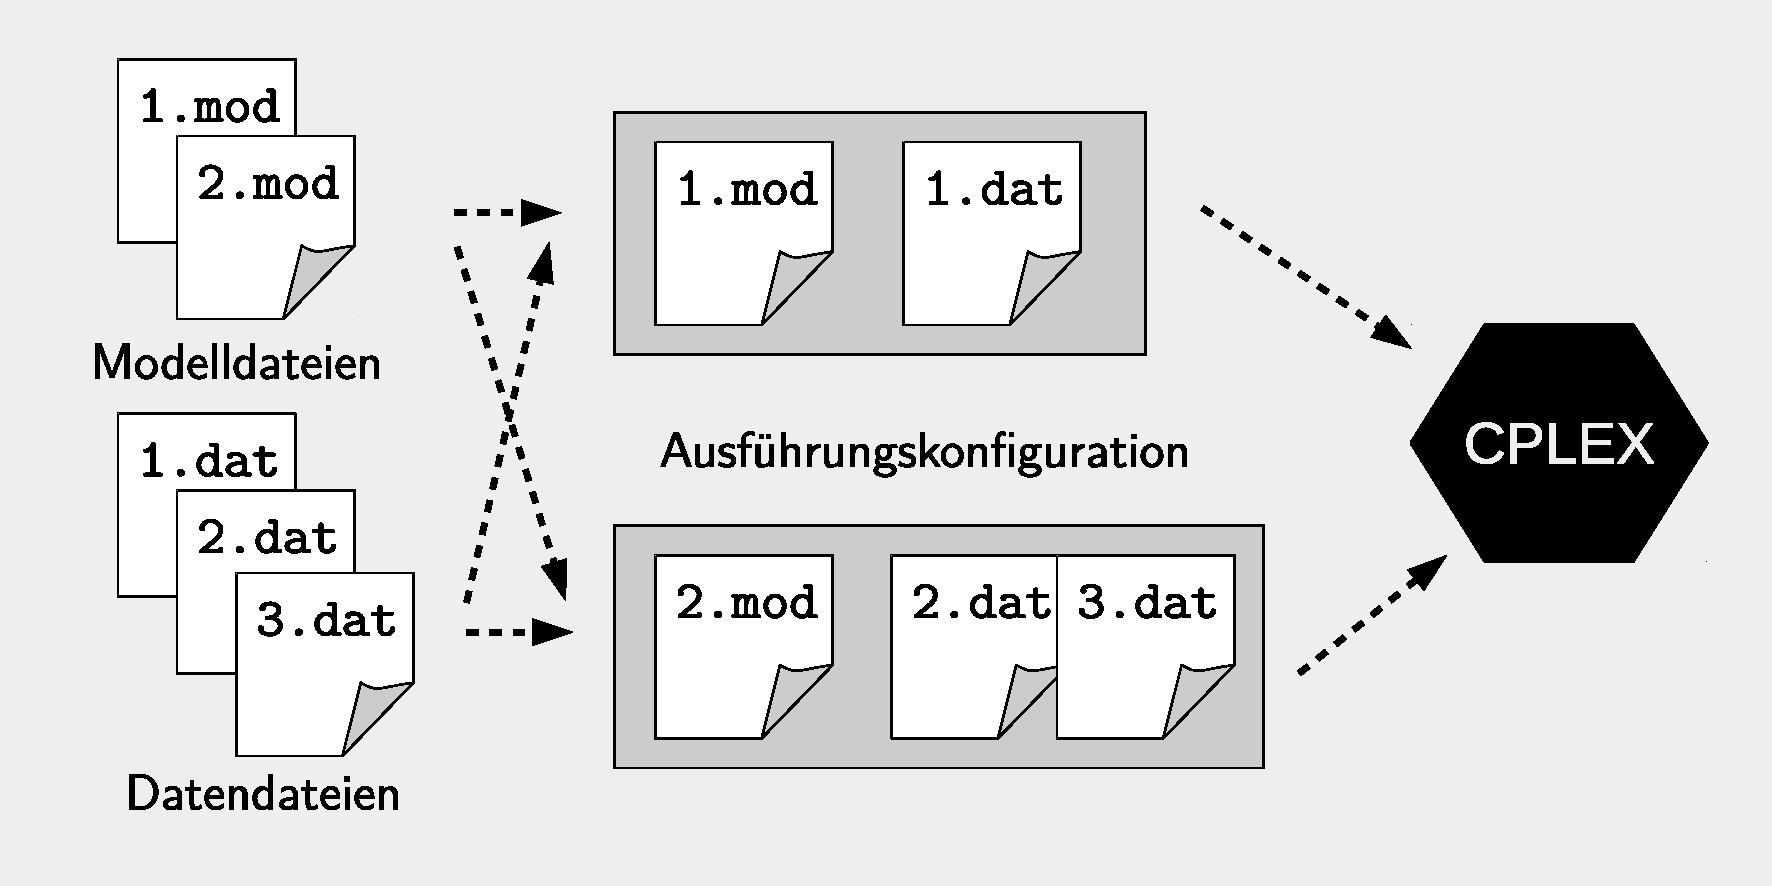
\includegraphics[width=\linewidth]{Bilder/OPL-Aufbau}
 \end{figure}
\end{frame}
